\chapter{Methodology}

\section{Research Design}
This thesis adopts a comparative experimental design to evaluate chest X-ray diagnostic classification under a controlled setting. The central goal is to determine whether transfer learning improves binary chest X-ray classification performance and whether explainability methods can make model behavior easier to interpret. To ensure that the comparison is fair, all experiments use the same dataset, label definition, preprocessing pipeline, split strategy, and evaluation metrics. The only differences between the core experiments are the network architecture and the training strategy.

Four main experiments are defined in this study. The first and second experiments use ResNet50, while the third and fourth experiments use DenseNet121. For each architecture, one model is trained from scratch and one model is trained with ImageNet-pretrained weights. This yields the following comparison structure:
\begin{itemize}
    \item ResNet50 trained from scratch;
    \item ResNet50 with transfer learning;
    \item DenseNet121 trained from scratch;
    \item DenseNet121 with transfer learning.
\end{itemize}
This design makes it possible to analyze two questions directly: whether one architecture is more suitable for the selected task, and whether transfer learning provides a consistent performance advantage across both architectures.

\section{System Workflow}
Figure \ref{fig:system-workflow} summarizes the end-to-end workflow used in this thesis. The pipeline begins with NIH ChestXray14 image-label pairs, applies binary label mapping and preprocessing, creates a fixed train-validation-test split, trains the four controlled model configurations, and then evaluates the final models using both quantitative metrics and Grad-CAM-based qualitative analysis. This workflow is intentionally simple so that the full comparison remains reproducible and easy to audit.

\begin{figure}[htbp]
    \centering
    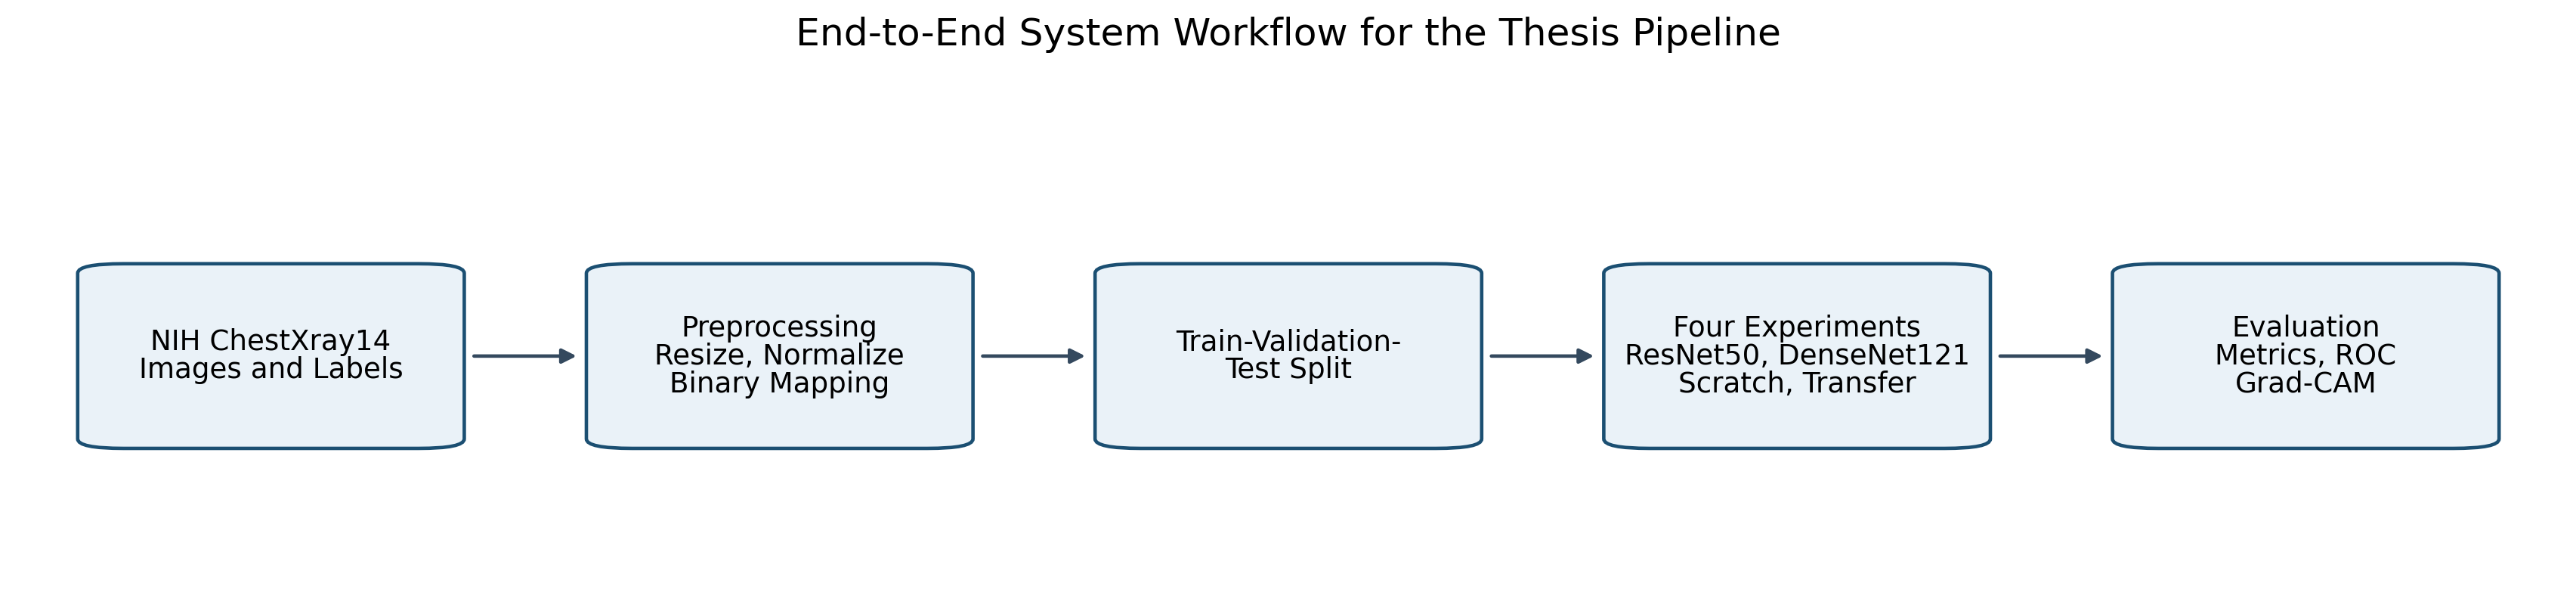
\includegraphics[width=\textwidth]{outputs/figures/thesis_revision/workflow_diagram.png}
    \caption{End-to-end workflow for the thesis pipeline.}
    \label{fig:system-workflow}
\end{figure}

\section{Dataset Description}
The experiments are based on the NIH ChestXray14 dataset, which is one of the most widely used public benchmarks for chest radiograph analysis \cite{ref:wang2017}. The dataset contains a large collection of frontal chest X-ray images with labels mined from radiology reports. Because the original dataset is multi-label and includes several thoracic disease findings, it is useful for many different classification settings. However, for the purpose of this capstone, the task is simplified to binary classification so that the effect of architecture choice, transfer learning, and explainability can be studied in a more controlled way.

In this thesis, all images labeled ``No Finding'' are assigned to the \textit{Normal} class. Images containing one or more pathology labels are assigned to the \textit{Abnormal} class. This mapping converts the original multi-label problem into a binary normal-versus-abnormal decision problem. The binary setting is a practical choice for three reasons. First, it reduces ambiguity in the learning objective. Second, it allows clearer interpretation of evaluation metrics such as sensitivity and specificity. Third, it is appropriate for a focused capstone project where the main goal is comparative analysis rather than full clinical deployment.

This label mapping should be interpreted with caution. The NIH ChestXray14 labels are mined from radiology reports rather than manually annotated for this exact binary task, so label noise is expected. In addition, ``No Finding'' does not necessarily mean that the patient is completely healthy; it only means that no corresponding abnormality was extracted from the associated report. Therefore, the \textit{Normal} and \textit{Abnormal} classes used in this thesis are operational research labels for a controlled experiment, not definitive clinical ground truth.

\section{Data Preprocessing}
The data preprocessing pipeline is designed to produce reproducible model inputs while preserving the overall structure of the chest radiographs. First, metadata are inspected to identify the image path, patient identifier if available, and original disease labels. After the binary label mapping is applied, the dataset is divided into training, validation, and test subsets using a target split ratio of 70\%, 15\%, and 15\%, respectively. If patient identifiers are available, patient-level splitting is used to reduce the risk of data leakage between training and evaluation sets.

All images are resized to $224 \times 224$ pixels so that they can be processed consistently by both ResNet50 and DenseNet121. Since chest X-ray images are grayscale but the selected pretrained models are designed for three-channel input, the image is converted into a model-compatible tensor format while preserving the underlying grayscale information. Pixel values are normalized after resizing so that training remains stable across different model configurations.

To reduce overfitting and improve robustness, training-time augmentation is applied to the training subset only. The final augmentation strategy includes resizing, normalization, and a modest set of geometric or intensity-preserving transformations that do not distort the clinical meaning of the radiograph. The validation and test sets use deterministic preprocessing only, so that the evaluation remains stable and comparable across runs. Every preprocessing step is documented so that the full experimental pipeline can be reproduced later.

\section{Model Architectures}
Two convolutional neural network architectures are used in this study: ResNet50 \cite{ref:he2016} and DenseNet121 \cite{ref:huang2017}. These models are selected because they are well established, widely used in medical image classification, and supported by pretrained ImageNet weights. They also provide a meaningful comparison between two influential design philosophies in convolutional neural networks.

ResNet50 is based on residual learning, where shortcut connections allow information to bypass one or more layers. This helps stabilize optimization in deep networks and makes residual models strong baselines across many vision tasks. In the context of this thesis, ResNet50 is included because it represents a mature and widely adopted architecture that can serve as a reliable benchmark.

DenseNet121 uses dense connectivity, in which each layer receives feature information from earlier layers in the same dense block. This design promotes feature reuse and improves gradient flow during training. DenseNet121 is especially relevant to chest X-ray analysis because it was used by CheXNet and has become one of the most recognizable baselines in this area \cite{ref:rajpurkar2017}. In all experiments, the final classification layer of each network is adapted to output the binary classes required by the selected task.

\section{Training Strategies}
Two training strategies are compared for each model. In the first strategy, the network is trained from scratch using random parameter initialization. In the second strategy, the network is initialized with ImageNet-pretrained weights and then fine-tuned on the target chest X-ray dataset. This comparison is motivated by prior medical imaging work showing that transfer learning often improves convergence and performance when labeled data are limited or noisy \cite{ref:tajbakhsh2016,ref:shin2016}.

The final training configuration used a batch size of 16, a learning rate of $10^{-3}$, the Adam optimizer, and \texttt{BCEWithLogitsLoss} for binary classification. Each experiment was trained for up to 20 epochs, and the best checkpoint was selected based on validation AUC. An early stopping mechanism with patience set to 5 was used to reduce unnecessary computation and to limit overfitting. The same optimization procedure was applied consistently across the four core comparisons.

The same learning rate was used across all experiments to preserve comparability between architectures and training strategies. This design choice keeps the comparison focused on architecture and initialization rather than on separately tuned hyperparameters. However, for pretrained CNN fine-tuning, a lower learning rate can sometimes be more appropriate. Separate learning-rate tuning for scratch and transfer-learning settings is therefore treated as a direction for future work rather than as part of the controlled comparison in this thesis.

For transfer learning, the pretrained model was adapted by replacing the original final classification head with a binary output layer and then fine-tuned on the target dataset under the same experimental conditions used for the scratch-training baseline. Weighted loss was not introduced into the four main comparisons because the goal of the thesis was to preserve a controlled comparison focused on architecture choice and training strategy.

\paragraph{Algorithmic procedure.}
The practical training procedure used throughout the thesis can be summarized as follows:
\begin{enumerate}
    \item Load the predefined training and validation splits and apply the corresponding transforms.
    \item Initialize either ResNet50 or DenseNet121 with scratch weights or ImageNet-pretrained weights.
    \item Replace the original classification head with a binary output layer.
    \item Train the model for one epoch using mini-batch Adam optimization and binary cross-entropy loss.
    \item Evaluate the model on the validation split and record validation AUC.
    \item Save the checkpoint if validation AUC improves; otherwise increment the early-stopping counter.
    \item Stop training when the patience limit is reached or the maximum number of epochs is completed.
\end{enumerate}

\section{Evaluation Metrics}
Model performance is evaluated using a set of standard binary classification metrics. These include accuracy, precision, recall, F1-score, and the area under the ROC curve (AUC). Accuracy measures overall correctness, while precision and recall provide complementary views of positive prediction quality and sensitivity to abnormal cases. F1-score is useful because it balances precision and recall, especially when class distributions are uneven. AUC is included because it measures ranking quality across decision thresholds and is frequently reported in chest X-ray studies \cite{ref:wang2017,ref:irvin2019}.

In addition to these summary metrics, confusion matrices are used to analyze false positives and false negatives. Sensitivity and specificity are also reported because they are especially meaningful in a diagnostic setting. Together, these metrics allow the thesis to compare models not only by final predictive performance but also by error behavior and class-specific tradeoffs.

The binary classification loss used in the experiments is \texttt{BCEWithLogitsLoss}, which combines a sigmoid activation with binary cross-entropy:
\begin{equation}
\mathcal{L} = -\frac{1}{N}\sum_{i=1}^{N} \left[y_i \log \sigma(z_i) + (1-y_i)\log \left(1-\sigma(z_i)\right)\right],
\end{equation}
where $z_i$ is the model logit for sample $i$, $\sigma(\cdot)$ is the sigmoid function, and $y_i \in \{0,1\}$ is the binary class label.

The main evaluation metrics are computed from the standard confusion-matrix counts true positive (TP), true negative (TN), false positive (FP), and false negative (FN):
\begin{equation}
\text{Accuracy} = \frac{TP + TN}{TP + TN + FP + FN},
\end{equation}
\begin{equation}
\text{Precision} = \frac{TP}{TP + FP},
\end{equation}
\begin{equation}
\text{Recall} = \text{Sensitivity} = \frac{TP}{TP + FN},
\end{equation}
\begin{equation}
F1 = \frac{2 \cdot \text{Precision} \cdot \text{Recall}}{\text{Precision} + \text{Recall}},
\end{equation}
\begin{equation}
\text{Specificity} = \frac{TN}{TN + FP}.
\end{equation}
The AUC is not tied to a single decision threshold; instead, it summarizes ranking quality across the full ROC curve by measuring how well abnormal cases are ranked above normal cases.

\section{Explainability with Grad-CAM}
Explainability is incorporated into the methodology through Grad-CAM \cite{ref:selvaraju2017}. After the quantitative evaluation is completed, Grad-CAM is applied to representative images from the test set in order to visualize which image regions most strongly influence model predictions. This process is used for both correctly classified and misclassified cases. By analyzing correct normal predictions, correct abnormal predictions, false positives, and false negatives, the study can examine whether the model focuses on plausible thoracic regions or relies on irrelevant patterns.

The purpose of Grad-CAM in this thesis is not to claim perfect interpretability, but to provide qualitative evidence about model behavior. This is particularly important in medical imaging, where an apparently strong model may still behave unreliably if its predictions are driven by spurious visual cues. Grad-CAM therefore complements the numerical results by supporting a focused error analysis and a discussion of model trustworthiness.

\section{Implementation Environment}
The implementation environment for this study is Python with standard deep learning and data analysis libraries. The core framework is PyTorch, supported by torchvision for pretrained model access and image transforms. Additional tools include NumPy and pandas for data handling, scikit-learn for evaluation metrics, and matplotlib for visualization. Model checkpoints, result tables, training logs, ROC curves, confusion matrices, and Grad-CAM figures are stored in the project workspace so that results can be reused directly in later chapters of the thesis.

Overall, the methodology is designed to balance rigor and feasibility. The project does not attempt to solve every problem in chest X-ray analysis. Instead, it uses a narrow but defensible experimental design to answer a focused research question: whether standard convolutional architectures, combined with transfer learning and Grad-CAM, can provide an effective and interpretable framework for binary chest X-ray diagnostic classification.
